\documentclass[11pt]{article}
\usepackage{amsmath,amsthm,amssymb,fullpage,graphicx,hyperref,listings}
\usepackage{listings,color,setspace}
\author{Andy Reagan}
\title{Math 337 Homework 14}

     \def\NN{\mathbb{N} }
     \def\ZZ{\mathbb{Z} }
     \def\QQ{\mathbb{Q} }
     \def\RR{\mathbb{R} }
     \def\CC{\mathbb{C} }
     \def\f{\frac }
     \def\b{\begin }
     \def\e{\end }
     \def\Log{\text{Log} \,}
     \def\Re{\text{Re} \, }
     \newcommand{\pdiff}[2]{\frac{\partial #1}{\partial #2}}
     \newcommand{\partialdiff}[2]{\frac{\partial #1}{\partial #2}}
     \newcommand{\pdiffsq}[2]{\frac{\partial^2 #1}{{\partial #2}^2}}
     \newcommand{\pdiffcu}[2]{\frac{\partial^3 #1}{{\partial #2}^3}}
     \newcommand{\pdiffhi}[3]{\frac{\partial^#3 #1}{{\partial #2}^#3}}
     \newcommand{\diff}[2]{\frac{{\rm d}#1}{{\rm d}#2}}
     \newcommand{\diffsq}[2]{\frac{{\rm d}^{2}#1}{{\rm d} {#2}^2}}
     \newcommand{\diffhi}[3]{\frac{{\rm d}^#3 #1}{{\rm d} {#2}^#3}}
     \newcommand{\tdiff}[2]{\mbox{d} #1/\mbox{d} #2}
     \newcommand{\tdiffsq}[2]{\mbox{d}^{2} #1/\mbox{d} {#2}^2}
     \newcommand{\tpdiff}[2]{\partial #1/\partial #2}
     \newcommand{\tpdiffsq}[2]{\partial^2 #1/\partial {#2}^2}
     \newcommand{\bvec}[1]{\vec{ {\bf #1 } }}
     \newcommand{\oh}[1]{O(h^{{#1}})}

\lstset{language=MATLAB,
basicstyle=\ttfamily\scriptsize\singlespacing,
keywordstyle=\color{black},
stringstyle=\color{black},
commentstyle=\color{black},
morecomment=[l][\color{black}]{\#},
frame=L,
xleftmargin=\parindent,
%%numbers=left,                   %% where to put the line-numbers
%%numberstyle=\scriptsize,      %% the size of the fonts that are used for the line-numbers
%%stepnumber=1,                   %% the step between two line-numbers. If it is 1 each line will be numbered
numbersep=5pt,
breaklines=true,        %% sets automatic line breaking
breakatwhitespace=false,    %% sets if automatic breaks should only happen at whitespace
escapeinside={\%*}{*)} 
}

%% example code insert
%% \lstinputlisting[language=Matlab]{andy_hw12_prb01.m}

%% example figure
%% \begin{figure}[h!]
%%   \centering
%%     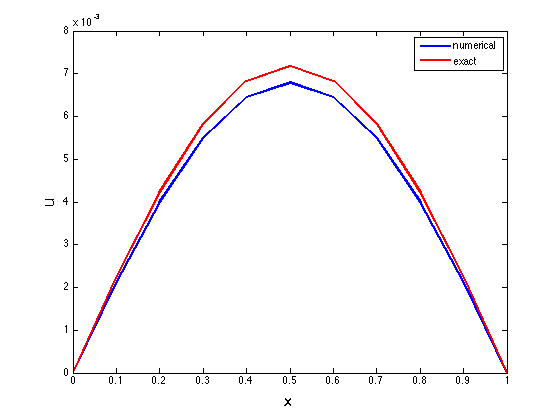
\includegraphics[width=0.45\textwidth]{andy_hw12_prb01_02.png}
%%   \caption{The numerical and exact solution for $h=0.1$.}
%% \end{figure}

%% start problem on next page
%% \clearpage
%% \pagebreak

\begin{document}
\maketitle

\begin{enumerate}

\item I solve the IBVP using method (14.10). To check the $u_x$ boundary condition is verified, we approximate
\begin{align*} u'_0 &= \f{u_1-u_0}{h} - \f{h}{2} u_0 '' + \oh{2}\\
&= \f{u_1-u_0}{h} -  \f{h}{2} \left ( \f{u_2 -2u_1 +u_0}{h^2} + \oh{1} \right ) + \oh{2}\\
&= \f{u_1-u_0}{h} -  \f{u_2 -2u_1 +u_0}{2h} + \oh{2} .\end{align*}

In addition to the solution at time $t=2$, I include a plot of the error in the numerical solution BC at $x = 0$, the mixed BC.

\lstinputlisting[language=Matlab]{andy_hw14_prb01.m}

\begin{figure}[h!]
  \centering
    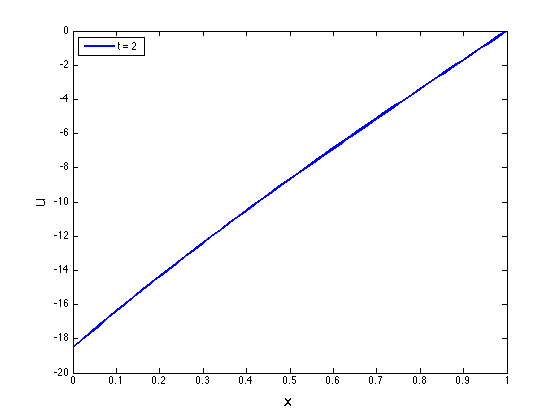
\includegraphics[width=0.45\textwidth]{andy_hw14_prb01_01.png}
  \caption{Solution of IBVP of Problem 1 using method 14.12.}
\end{figure}

\begin{figure}[h!]
  \centering
    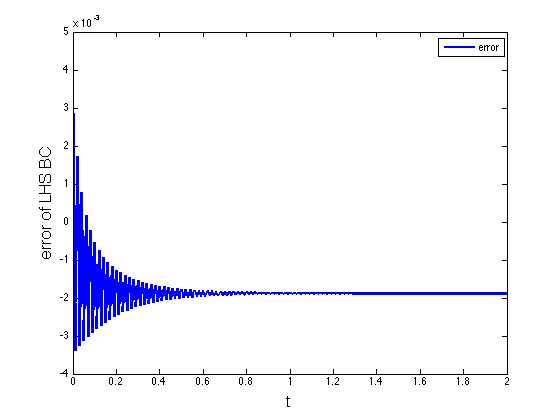
\includegraphics[width=0.45\textwidth]{andy_hw14_prb01_03.png}
  \caption{Error in the BC at $x=0$ of the numerical solution of IBVP of Problem 1 using method 14.12.}
\end{figure}

\item The numerical scheme (14.19), upon plugging in for $\delta _x ^2$ and $\delta _t$ becomes (gathering terms in $U_i ^j$, and letting $\gamma = 1$):
\begin{align*} &U_{m+1} ^{n+1} \left ( -\f{r}{2} \alpha _{m+1/2} ^{n+1} +\f{r}{2} \alpha _{m-1/2} ^{n+1} \right ) + U_{m} ^{n+1} \left ( 1 - \f{\kappa}{2} \beta _{m} ^{n+1} +r \alpha _{m+1/2} ^{n+1} -r \alpha _{m-1/2} ^{n+1} \right )\\
&~~~~ + U_{m+1} ^{n+1} \left ( \f{r}{2} \alpha _{m+1/2} ^{n+1} -\f{r}{2} \alpha _{m-1/2} ^{n+1} \right )\\
&~~~~ = U_{m+1} ^{n} \left ( \f{r}{2} \alpha _{m+1/2} ^{n} -\f{r}{2} \alpha _{m-1/2} ^{n} \right ) + U_{m} ^{n} \left ( 1 + \f{\kappa}{2} \beta _{m} ^{n} -r \alpha _{m+1/2} ^{n} +r \alpha _{m-1/2} ^{n} \right )\\
&~~~~ + U_{m+1} ^{n} \left ( - \f{r}{2} \alpha _{m+1/2} ^{n} +\f{r}{2} \alpha _{m-1/2} ^{n} \right )\end{align*}

\lstinputlisting[language=Matlab]{andy_hw14_prb02.m}

\begin{figure}[h!]
  \centering
    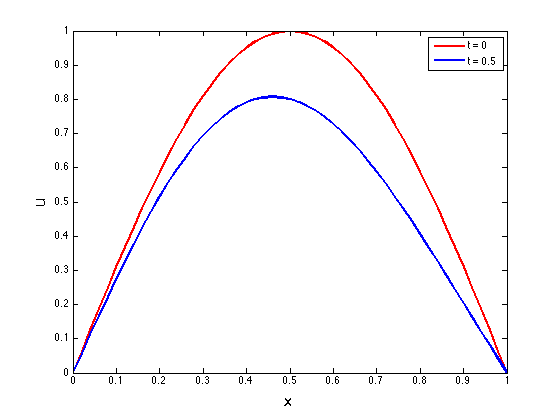
\includegraphics[width=0.45\textwidth]{andy_hw14_prb02_01.png}
  \caption{Solution of IBVP of Problem 2 using method 14.19.}
\end{figure}

\item Applying the Von Nuemann stability analysis, we have
\[ \f{U_{m+1} ^{n+1}-2U_{m} ^{n+1}+U_{m-1} ^{n+1}}{h^2} = \f{3}{2} \f{U_{m} ^{n+1}-U_{m} ^{n}}{\kappa} - \f{1}{2} \f{U_{m} ^{n} - U_{m} ^{n-1}}{\kappa}. \]
Letting $r = \kappa/h^2$, 
\[ 2r \left ( U_{m+1} ^{n+1}-2U_{m} ^{n+1}+U_{m-1} ^{n+1}\right )  = 3\left ( U_{m} ^{n+1}-U_{m} ^{n} \right )  + \left ( U_{m} ^{n} - U_{m} ^{n-1} \right ), \]
and since this in linear, we replace $U$ with the error $\epsilon$ 
\[ 2r \left (\epsilon_{m+1} ^{n+1}-2\epsilon_{m} ^{n+1}+\epsilon_{m-1} ^{n+1}\right )  = 3\left ( \epsilon_{m} ^{n+1}-\epsilon_{m} ^{n} \right )  - \left ( \epsilon_{m} ^{n} - \epsilon_{m} ^{n-1} \right ), \]
Now we expand $\epsilon$ with a specific Fourier series, namely $\epsilon \to \rho ^n e^{i\beta m h}$:
\begin{align*} 2r \left (\rho ^{n+1} e ^{i \beta (m+1) h}-2\rho ^{n+1} e ^{i \beta (m) h}+\rho ^{n+1} e ^{i \beta (m-1) h}\right )  &= 3\left ( \rho ^{n+1} e ^{i \beta (m) h}-\rho ^{n} e ^{i \beta (m) h}\right ) \\
&~~~~- \left ( \rho ^{n} e ^{i \beta (m) h} - \rho ^{n-1} e ^{i \beta (m) h} \right ). \end{align*}
Cancelling $\rho ^{n-1} e^{i\beta m h}$, we are left
\begin{align*} 2r \left (\rho ^{2} e ^{i \beta h}-2\rho ^{2} +\rho ^{2} e ^{-i \beta }\right )  = 3\left ( \rho ^{2} -\rho \right )- \left ( \rho - 1\right ). \end{align*}
Finally, I collect the remaining exponentials in to a cosine term, and we have
\begin{align*} 4r\rho ^{2} \left ( \cos (\beta h)-1\right )  = 3\rho \left ( \rho -1\right )- \left ( \rho - 1\right ) = 3\rho ^2 -4\rho +1 . \end{align*}
Which is
\begin{align*} 4r\rho ^{2} \left ( \cos (\beta h)-1\right )  - 3\rho ^2 +4\rho -1  = 0. \end{align*}
Although we could simplify this and plot in 2D, it is simpler just to look at the magnitude of $\rho$ versus a reasonable range of $r$ and $\beta h$ independently.
Now we turn to plotting the largest magnitude root $\rho$ for $\beta h \in [0,\pi]$ and $r \in [0,10]$.
The following code does just that:

\lstinputlisting[language=Matlab]{andy_hw14_prb03.m}

\begin{figure}[t!]
  \centering
    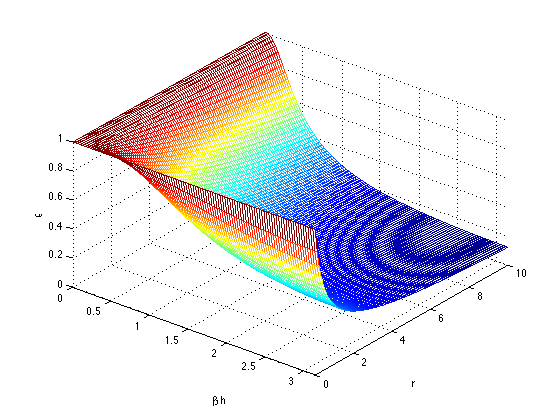
\includegraphics[width=0.45\textwidth]{andy_hw14_prb03_01.png}
  \caption{Magnitude of the largest root $\rho$ in the Von Nuemann stability analysis of the scheme of Problem 3.
  We observe unconditional stability, since the largest root $\rho$ has magnitude less than one for $\beta h \ne 0, r\ne 0$.}
\end{figure}

It appears that this method will better smooth a discontinuous initial condition, since for $\beta h$ close to 0, (the highest frequency mode), this method has $\rho$ drop off more quickly than the CN method.

\item To solve the nonlinear IBVP, I first attempt using the semi-implicit method described by Eq. 14.50 of the notes.
The main reason that I attempt this first is that the Newton-Raphson looks cumbersome to code.



\end{enumerate}
\end{document}



